\documentclass{llncs} 

\usepackage{verbatim}
%\usepackage[pdfpagescrop={92 112 523 778},a4paper=false]{hyperref}
\usepackage{hyperref}
\usepackage[pdftex]{graphicx}
\hypersetup{
    pdftitle={FOAF+SSL: RESTful Authentication for Distributed Social Networks},
    pdfauthor={Bruno Harbulot, Ian Jacobi, Henry Story, Mike Jones},
    pdfkeywords={}
}

\graphicspath{{figures/}}
\urlstyle{sf}

\usepackage[hyper]{listings}
\lstset{basicstyle=\rm\footnotesize\ttfamily,frame=tbrl,showstringspaces=false,columns=fixed,basewidth=0.55em}

\sloppy
\clubpenalty=50000
\widowpenalty=50000

%% To comment out for the final version
\newcount\hour
\newcount\minute
\def\Time{\hour=\time
          \minute=\time
          \divide\hour by60
          \ifnum\hour<10 0\fi\number\hour:%
          \multiply\hour by60
          \advance\minute by -\hour
          \ifnum\minute<10 0\fi\number\minute%
         }
\RequirePackage{rotating}
\RequirePackage{graphicx}
\RequirePackage{prelim2e}[1996/01/01]
\renewcommand*{\PrelimText}{%
	\hskip -1.2cm plus -\marginparsep
    \begin{rotate}{90}
       \rlap{%
          \scalebox{0.75}{\textnormal{\texttt{Draft: \today\ -- \Time -- Page \thepage}
          This article is available under the ``Attribution 3.0 Unported'' Creative Commons License.}}
       }%
    \end{rotate}
    \hskip 0pt plus 1filll
 }
%%%%%%%%%%%%%%%%%%%%%%%%
\newcounter{custompropcounter}
\newenvironment{customprop}[1]
{\refstepcounter{custompropcounter}\label{#1}%
\vspace{0.31cm}
\tabular{p{.08\textwidth}p{.91\textwidth}}
{\bf (P\arabic{custompropcounter})} & 
\minipage{\textwidth}
\footnotesize}
{\endminipage
\endtabular\vspace{0.31cm}}

\newcounter{customrelcounter}
\newenvironment{customrel}[1]
{\refstepcounter{customrelcounter}\label{#1}%
\vspace{0.31cm}
\tabular{p{.08\textwidth}p{.91\textwidth}}
{\bf (R\arabic{customrelcounter})} & 
\minipage{\textwidth}
\footnotesize}
{\endminipage
\endtabular\vspace{0.31cm}}

\newcounter{customdefcounter}
\newenvironment{customdef}[1]
{\refstepcounter{customdefcounter}\label{#1}%
\vspace{0.31cm}
\tabular{p{.08\textwidth}p{.91\textwidth}}
{\bf (D\arabic{customdefcounter})} & 
\minipage{\textwidth}
\footnotesize}
{\endminipage
\endtabular\vspace{0.31cm}}


\begin{document}
\title{FOAF+SSL: RESTful Authentication for Distributed Social Networks}
\author{Henry Story\inst{1} \and Bruno Harbulot\inst{2} \and Ian Jacobi\inst{3} \and Mike Jones\inst{2}}
\institute{Sun Microsystems, 
\url{http://blogs.sun.com/bblfish}
\and
The University of Manchester, UK,
\email{Bruno.Harbulot@manchester.ac.uk}
\and
MIT}

\maketitle
\begin{abstract} 
 We describe a very simple protocol for RESTful authentication, using
 widely deployed technologies such as HTTP, SSL/TLS and Semantic Web
 vocabularies.  This protocol can be used for one click sign on to web sites - 
 without requiring the user to enter an identifier or password - using existing 
 browsers, and for distributed open yet secure social networks. 
 After describing each of these technologies and how
 they come together in FOAF+SSL\footnote{Up-to-date information on
   developments in this protocol are available at
   \url{http://esw.w3.org/topic/foaf+ssl}.}, we show declaratively the
 reasoning of a server relying on this authentication mechanism to
 make authorization decisions.
\end{abstract}
\section{Introduction}

Many services that require authentication rely on centralized systems
(usually backed by an LDAP database).  The identity of the user is restrained
to that administrative domain, forcing her to have a different account and identifier
for each organization she interacts with. This inability to related identities easily accross
domains also makes the creation of links between  users in distinct organizations 
difficult. 

Every time a new user needs authenticated access to a new
organization, a new registration needs to be made; this is a burden
for both the user and the organization. The process of registration is
either (a) minimal ---for example, e-mail address confirmation---, or
(b) more formal ---for example, in a workplace, where an
administrator has to create an account, after verifications
out-of-band. Process (a) is lightweight, but will often provide
insufficient information, whereas process (b) may initially be able to give more
information about a user, at the expense of a costly
verification phase during the registration.

Attempts to decentralize this process have been
made. Shibboleth,\footnote{\url{http://shibboleth.internet2.edu/}} for
example, aims at sharing accounts across administrative boundaries;
however, it relies on a rigid federation process between
organizations.  OpenID, enables authenticating a user against a URI,
but requires a separate protocol and the definition of custom
attributes for obtaining more information about the user.  Neither
Shibboleth nor OpenID fully comply with the Web Architecture
Principles (REST), thereby making it difficult to gain extra
information about a user in the decentralized, hyperlinked ways of the
Web.

This paper proposes a novel approach which relies on combining the use
of SSL client certificates and Semantic-Web-based FOAF networks. The
result is a secure, open and distributed authentication mechanism,
which is able to satisfy simple requirements ---such as authenticating
a user by URI, like OpenID--- and more complex requirements, where the
authorization to a service depends on knowledge of the position in the
social network of the authenticating agent, as inferred from documents
containing FOAF and other Semantic Web relations. This is made
possible by a RESTful architecture, the same that underpins the
largest and most successful network of distributed linked information:
the Web.

Section~\ref{sec:background} introduces the background technologies of
the Semantic Web and FOAF, as well as cryptography and
client-certificate authentication.  Section~\ref{sec:foaftlsprotocol}
presents the FOAF+SSL protocol.  Section~\ref{sec:other} compares this
approach to others.

\section{Background}
\label{sec:background}

\subsection{The RESTful Web Architecture}
\label{sec:rest}

{\em Representational State Transfer} ({\em
  REST})~\cite[Chap.~5]{fielding2000phd} is an architectural style for
building large-scale distributed information networks, the most famous
of these being the World Wide Web~\cite{WebArchVol1}.  To build such a
network requires that each of the parts be able to grow independently
of any of the others, with close to no central coordination, and that
each of the resources thus created be able to refer easily to any of
the others, in a seamless manner.

The logical building blocks for this are the following:
\begin{enumerate}
\item The specification of universal names, also known as Universal
  Resource Identifiers (URI) --- the best known being the subset
  called Universal Resource Locators (URLs).
\item The mapping of URIs to Resources. This is the reference part of
  the semantic piece.
\item Canonical methods for manipulating these resource mapped by each
  URIs, via {\em representations} of the resource.  Such a protocol
  specifies a canonical dereferencing mechanism, enabling a holder of
  a URI to find and manipulate the resource referred to by that URI.
  {\tt http://...} URLs use the HTTP protocol as their dereferencing
  mechanism, for example.  By accessing the object at a given HTTP
  URL, information about the resource, known as the {\em
    representation} of the resource, can be fetched.  The resource can
  be changed if permitted -- including here creation or deletion as
  limiting cases.
\end{enumerate}

REST specifies the architectural style required for building such a
protocol, with the aim of maximum networkability; that is, any
representation should be able to link to any resource from anywhere
using the URI alone to do so. Moreover, any user should be able to
reach any part of the system in such a way.

\subsection{The Semantic Web}

Whereas URLs in the initial web of hyperlinked documents referred only
to documents, the Semantic Web specifies how to extend this to enable
a web of interlinked resources. In the Semantic Web, it becomes
possible for URLs to refer to anything, be it:
\begin{enumerate}
\item concrete things like individual people --- e.g. {\tt
  <https://romeo.example/\#i>}\footnote{Following RFC2606\cite{rfc2606} we use the {\tt .example} top-level
  domain to highlight URLs that are not dereferenceable and are being used as examples here.} refers to
  a human named Romeo;
\item relations between two individuals --- e.g. the relation of
  knowing someone which {\tt <http://xmlns.com/foaf/0.1/knows>} refers
  to;
\item or classes --- e.g. the set of people: {\tt
  <http://xmlns.com/foaf/0.1/Person>}.
\end{enumerate}

The meaning of these URLs can be found by dereferencing them using
their canonical protocol. Thus, doing an HTTP GET on {\tt
  <\url{http://xmlns.com/foaf/0.1/knows}>} should return a
representation describing it. As HTTP is built to allow content
negotiation, clever web servers will return the representation best
fitting the client's needs. Entering the above URL in a web browser
will return a human readable web page describing the `knows'
relation. A Semantic Web agent could ask for the standard
machine-friendly RDF/XML representation and parse it; yet other
representations could be returned to describe the same information.

A semantic web document is a serialization of a graph of directed
relations between objects. Each relation exists as a triple of {\tt
  <subject> <relation> <object>}, where each of {\tt subject}, {\tt
  relation} and {\tt object} can be chosen among any of the URIs, and
{\tt object} may also be a string literal. As it is tedious to read
and write such URLs, this article uses the N3\footnote{Current N3
  tutorial at:
  \url{http://www.w3.org/2000/10/swap/doc/Overview.html}.} {\tt
  @prefix} notation. The following prefixes will be used throughout
this article:

\begin{lstlisting}[basicstyle=\rm\scriptsize\ttfamily]
@prefix log: <http://www.w3.org/2000/10/swap/log#> .
@prefix dc: <http://purl.org/dc/elements/1.1/> .
@prefix cert: <http://www.w3.org/ns/auth/cert#> .
@prefix rsa: <http://www.w3.org/ns/auth/rsa#>
@prefix foaf: <http://xmlns.com/foaf/0.1/> .
@prefix rdfs: <http://www.w3.org/2000/01/rdf-schema#> .
@prefix owl: <http://www.w3.org/2002/07/owl#> .
@prefix romeo: <https://romeo.example/#> . 
@prefix jult: <https://juliet.example/#> . 
@prefix : <> . # special vocabulary defined for this paper 
\end{lstlisting}

Thus, to say ``Romeo is a person'', one can write: {\tt romeo:i a foaf:Person.}

Each representation returned by a resource can be interpreted as a
graph of relations, which can be isolated in N3 by placing them within
curly brackets \{ \}.\footnote{These are similar to the Named Graph curly
brackets in SPARQL, except that the N3 notation allow anonymous graphs.}  The
relation that maps a resource to the graph described by the document retrieved using the
canonical dereferencing method of its URI  is defined as the {\tt :semantics} relation. Thus,
starting with the {\tt romeo:i} URL, one can, after dereferencing it,
state the following, without being obliged to explicitly assert the
actual statements within the brackets as true:

\begin{customprop}{prop:romeoSem}
\begin{verbatim}
	romeo:i :semantics { romeo:i a foaf:Person;
	                             foaf:name "Romeo";  
	                             foaf:knows  jult:me . }
\end{verbatim}
\end{customprop}


%Of special note here is the introduction of curly-brackets to the more
%familiar syntax of N-Triples or Turtle. 
%In particular, curly-brackets are used to enclose a particular graph of triples such that the graph may be
%related to other properties.

These graphs can also be used to formulate rules as when we define the
above {\tt :semantics} relation in terms of the established {\tt
  log:semantics} which relates a document to its graph, and {\tt :representation} 
relating a resource to one of its representations:

\begin{customdef}{def:representation}
\begin{verbatim}
	{ ?resource :representation ?doc . ?doc log:semantics ?graph . } 
	      => { ?resource :semantics ?graph . }
\end{verbatim}
\end{customdef}


The {\tt log:} namespace\footnote{The {\tt log:} namespace is
  described at \url{http://www.w3.org/DesignIssues/N3Logic}.} tends to
make significant use of enclosed graphs, or ``formulas''. Some worth mentioning
for this paper are the {\tt log:includes} property, which links a subject graph to an object
graph by asserting that the latter is a subset of the former graph, or
the {\tt log:implies} property, also written as {\tt =>}, which can
serve as the basis for reasoning based on first-order logic (with the
introduction of appropriate variables).

Even though the Semantic Web is built in order to make merging of
information easy, it is not a requirement to do so. We will be using
this notation to help illustrate clearly when and for what reason
merging graphs is reasonable.

\subsection{FOAF, reputation networks and the Web of Trust}

{\em FOAF},\footnote{Defined at \url{http://xmlns.com/foaf/0.1/}.}
short for Friend-of-a-Friend, is an RDF vocabulary used to describe
people, agents, groups and their relations in a practical way. When
used on the Semantic Web, this allows each person to describe his
network of friends.

By giving oneself a URI --~{\em aka.} a WebId -- one can describe one's
personal social network by linking oneself to one's acquaintances by
reference.  Consider someone who had been given the {\tt romeo:i} URL
by Romeo himself, and had then fetched its {\tt :semantics}, ending up with the
statements  P\ref{prop:romeoSem}. He has
good reason to trust that the information there is correct,
and thus to merge it (in a defeasible manner) with his own belief
store, in order to act on it.
That graph itself will contains further URIs such as {\tt
  jult:me}, whose {\tt :semantics} the agent can also GET. The thought then is that, if {\tt romeo:i}
uses a URI, it is because he means to refer objectively to some thing further described 
by that URI's {\tt :semantics}. Similarly the user can then add {\tt romeo:i} to his foaf file, to publish
{\tt :me foaf:knows romeo:i}.

If the advantages gained by keeping information up-to-date is large
enough, a peer-to-peer information network arises, where each person
specializes in keeping up-to-date the information they feel
responsible for, linking to the best sources for objects he or she
does not wish to maintain. In return, as the quality
of one's information and links increases, others feel more confident
linking to it. There is an incentive to link to existing resources:
less work maintaining that information. 

As the network grows so the
value of the network grows exponentially, as predicted by Metcalf's
Law~\cite{SemWebMetcalf}, creating a virtuous circle.  Current social 
networking sites such as Facebook and LinkedIn, and older ones such
as eBay with its  transaction voting mechanism,  have shown how this can work 
in less distributed settings, but taking advantage of the same law.

The plain {\tt foaf:knows} relations could be enhanced with trust descriptions so as to create a {\em
  reputation network}~\cite{DBLP:conf/www/GolbeckPH03}, and, in the
case of FOAF+SSL, this trust can be backed by the use of cryptographic
keys and signatures, so as to form a secure Web of Trust (as described
in the next sections).

\subsection{Public key cryptography}

{\em Public key cryptography} allows two peers to communicate securely
without requiring them to share a secret.  It achieves this through
the use of unique pairs of keys.  One key, called the {\em public
  key}, may be disseminated widely, and the other, the {\em private
  key}, is generally held only by the person who generated the
key-pair.  This is in contrast to symmetric cryptography, where both
participants must share the knowledge of the same {\em secret} key for
both encryption and decryption.

Public key cryptography relies on the conjecture that it is infeasible
to obtain any private key that corresponds to a given public key
through brute force in a reasonable amount of time, because this
operation is too computationally expensive.  It also assumes that no
two distinct individuals will generate the same key-pair randomly. This
leads to defining {\tt hasPrivateKeyFor} as an inverse functional
property, in Definition D\ref{def:hasPrivateKeyFor}.

\begin{customdef}{def:hasPrivateKeyFor}
\begin{verbatim}
     :hasPrivateKeyFor a owl:InverseFunctionalProperty;
        rdfs:domain foaf:Agent;
        rdfs:range cert:PublicKey .
\end{verbatim}
\end{customdef}

Thanks to the dual-nature of the public and private key pair, two
distinct actions are made possible:

\begin{enumerate}
\item
{\em Encryption} is the obfuscation of a plain text message into a
scrambled message using the public key of a public/private key-pair,
so that it may only be decrypted using the corresponding private key,
ensuring that communications may not be decrypted by any other
recipient than the one intended.

\item
{\em Signing} is the process of associating a digital signature with a
message; this signature is generated using a private key. The
authenticity and integrity of the message can then be verified using
the corresponding public key.
\end{enumerate}

A {\em public key certificate} is the signed combination of a public
key and some information related to this key. Such a certificate may
be self-signed (using the private key that matches the public key it
contains) or signed by a third party.

A self-signed certificate allows the owner of a key pair to make
assertions about himself or herself.  Similarly a certificate signed by a
third party enables that party to endorse the contents of the certificate. If that third 
party is deemed trustworthy, that can be a reason for believing the contents too.

Two different architectures have been developed to make use of third
party signing of public key certificates: the hierarchical Public Key
Infrastructure (Section~\ref{sec:pkix}) and the cryptographic Web of
Trust (Section~\ref{sec:wot}).  In both architectures, an application
or hosting environment is initially configured with a trusted set of
certificates known as {\em trust anchors}.  When presented with an
unknown certificate, an application verifies the authenticity of the
certificate by attempting to build a certification path -- or chain --
between the certificate and one of the trust anchors. A certificate
becomes trusted if and only if it has been signed using a certificate
which is already trusted. If necessary, this operation may be repeated
to build a path through intermediate certificates, through which the
trust relation is transitive.

%Usually, the successful verification of a new certificate
%implies the establishment of only a temporary level of trust of the other party for the duration of some operation performed with the certificate. Applications may also, through some external mechanism,
%add some certificate to their set of trust anchors explicitly.

The hierarchical Public Key Infrastructure model and the cryptographic
Web of Trust model mainly differ in the way in which certificates are
distributed and intermediates are trusted. In both cases, the initial
establishment of trust (i.e. the selection of trust anchors) requires
an initial import of certificates which is out of band, but this
process is much less onerous than obtaining all public key
certificates for all entities likely to take part in secure
communications.


\subsection{PKI and hierarchical model of trust}
\label{sec:pkix}

The {\em Internet X.509 Public Key Infrastructure}~\cite{rfc5280}
(PKI) is a hierarchical model for distributing and trusting
certificates. In this model, certificates are signed by a {\em
  certification authority} (CA). X.509 certificates incorporate a {\em
  Subject Distinguished Name} (Subject DN), which identifies the
subject of the certificate, and an {\em Issuer Distinguished Name}
(Issuer DN), which identifies the issuer of the certificate. An X.509
certificate may only have one issuer DN, which must be the Subject DN
of the certificate that has been used to issue it (which consists of
signing it using the private key corresponding to the issuer
certificate). This structure builds a hierarchical tree from the root
CA certificate, via optional intermediate CA certificates, to the
end-entity (i.e. client or server) certificates.

The repository of trust anchors may have different names depending on
the platform and application. In practice, most web-browsers and
operating systems provide a default list of CA certificates (which
they make their users trust implicitly). This list can usually be changed
by the user, in order for example to add, replace or delete CA certificates. This
is widely used in corporate or institutional PKIs.

\subsection{Web of Trust}
\label{sec:wot}

The cryptographic {\em Web of Trust} (WoT) is a form of public key
infrastructure (although almost never called PKI) where each
participant may assert trust in any other participant, without a
specific hierarchy.

The Web of Trust model is used by PGP. What is often referred to as a
{\em PGP public key} is, in fact, a form of a public key certificate,
since it also contains additional information (such as an e-mail
address) and is signed so as to assert its authenticity. Such a
certificate is self-signed, but may also contain additional signatures
-- those by whom the association between the key and this additional
information is trusted.

In PGP, the trust anchors are the user's own certificate and the
certificates the user trusts, some of which may be from trusted
introducers (that is, people through whom trust is transitive).

Key-signing parties are often used for adding new trust anchors.  If a
participant, $A$, checks the identity of participant $B$, then $A$ may
opt to sign $B$'s certificate, thus asserting to $A$ and to any third
party who may have $A$ as a trusted introducer that the information in
$B$'s certificate is accurate.  Furthermore, direct trust may now be
established in future communications between $A$ and $B$ through the
use of public-key encrypted communications between $A$ and $B$.

If $A$ also trusts $B$ to make reasonable decisions in what
certificates $B$ signs, $A$ can also add $B$ as a trusted introducer,
so that $A$ can trust the certificates that $B$ has
signed. Furthermore, as more people sign $B$'s certificate, it becomes
more likely that a third party will be able to find a certification
path from themselves to $B$ via a chain of trusted introducers. To
make distribution of keys more practical, these certificates --signed
by as many people as possible-- may be stored on public key servers.

\subsection{SSL authentication}
\label{sec:tlsauth}

The most widely deployed protocol for securing communications between
a user-agent and a web server is Transport Layer Security
(TLS)~\cite{rfc2246}, itself a successor to the Secure Socket Layer
3.0 (SSLv3) specification;\footnote{Unless explicitly noted, this
  article uses SSL to encompass TLS 1.x and SSL 3.0.} its use in HTTP
applications is denoted by the {\tt https} prefix in URLs.

%TLS enables both secure transport of informations, as well as allowing client to identify the remote party.

%X.509 certificates are almost exclusively used to authenticate the remote party,
%even if TLS allows for other means of authenticating the communicating parties
%---for example using other types of certificates (see~\ref{sec:openpgpcipher})
%or Kerberos~\cite{rfc2712}.

When establishing an SSL connection, as part of the SSL handshake, the
client obtains an X.509 certificate from the server.  At this point,
the client relies on its trust anchors to verify it. If this
certificate is trusted and verified, the handshake proceeds. Once the
handshake has completed, the communication (on top of SSL) can proceed
in a secure manner; the only other party capable of reading the
communication must have the private key corresponding to this server
certificate.

There exists a variant of the handshake procedure in which the client
is requested or required to present a certificate to the server,
enabling the server to authenticate the client using the same
verification method as above.

The remainder of this section describes, from a Semantic Web point of view, what follows this handshake. This forms the basis for comparison of how FOAF+SSL differs from this, in Section~\ref{sec:authlogic}.

The following describes the reasoning of a server, {\tt S}, for
authenticating a client, {\tt \_:client}, making a request. Server
{\tt S} has a set of trusted CAs. {\tt S} would state that {\tt
  issuerDN} was a trusted CA with:

\begin{customprop}{def:trustedanchor}
\begin{verbatim}
   issuerDN a :TrustedCA;
            :hasPrivateKeyFor CAKey .
\end{verbatim}
\end{customprop}

The {\tt CAKey} is a {\tt cert:PublicKey} that is usually identified
by a number of inverse functional properties, which form an OWL2
key.\footnote{\url{http://www.w3.org/TR/owl2-syntax/\#Keys}} For the
sake of brevity, these relations are not shown here. Suffice it to say
that CA Keys can be uniquely identified by them.

{\tt S} requests that {\tt \_:client} presents a certificate signed by
any one of a number of CAs it knows about. {\tt S} receives {\tt
  \_:certDoc} with semantics such as the following (the subject is
also identified via a DN):

\begin{customprop}{prop:certcontent}
\begin{verbatim}
 _:certDoc :semantics _:certSemantics .
 _:certSemantics = { <> dc:created issuerDN ; foaf:primaryTopic subjectDN .
                     subjectDN :hasPrivateKeyFor pubKey .
                     issuerDN :hasPrivateKeyFor CAKey .  } 
\end{verbatim}
\end{customprop}

So far, the SSL handshake ensured {\tt S} that the client has the
private key:

\begin{customprop}{prop:clientcert}
\begin{verbatim}
    _:client :hasPrivateKeyFor pubKey .
\end{verbatim}
\end{customprop}

The client asserts the content of the certificate (not shown). It also
claims it is signed by {\tt issuer}:

\begin{customprop}{prop:clientclaim}
\begin{verbatim}
  _:client :claims  { _:certDoc :signature _:certSig;
                     _:certsig :signedWith CAKey; :sigString "XYZ SIG" ] . }
\end{verbatim}
\end{customprop}

{\tt S} can assert, after verification, that {\tt \_:certDoc} has been
signed using the private key corresponding to {\tt CAKey}:

\begin{customprop}{prop:sigverif}
\begin{verbatim}
_:certDoc :signature [ :signedWith CAKey ] .
\end{verbatim}
\end{customprop}

Proving that a document is signed by $P$, is to assert $P$ claims its
contents are true:

\begin{customdef}{def:signedCertClaim}
\begin{verbatim}
  {  ?P :hasPrivateKeyFor ?key .
     ?doc :signature [ :signedWith ?key ]
  } => {  ?P :claims [ is :semantics of ?doc ] } . 
\end{verbatim}
% Made change here.  Previously read ``?P claims that there exists
% some object that is the log:semantics of ?doc''.  I assume we meant
% ``?P actually claims the log:semantics of ?doc'', not ``?P believes
% there exists SOMETHING that is the log:semantics of ?doc'' (the
% latter of which is given from the definition of log:semantics, and
% hence meaningless to us).  This makes the following work properly,
% rather than asserting (the arguably correct, but misguided) ``issuer
% claims { [ is log:semantics of _:certDoc ] }.  This mostly keeps
% syntax correct at a bare minimum (object of ``claims'' is a
% formula.) -- Pipian
% 
% I disagree. P claims [ is log:semantics of ?doc ] .
% is equivalent to 
%    P claims _:s .
%    ?doc log:semantics _:s .
% notice the use of [ ] in the above. I we had used
% P claims { [] is log:semantics of ?doc }
% Pipian's point would hold -- Henry
\end{customdef}

Then, from the signature verification P\ref{prop:sigverif}, the
certificate contents P\ref{prop:certcontent} and the definition
D\ref{def:signedCertClaim}, {\tt S} can assert:

\begin{customprop}{prop:certcontent2}
\begin{verbatim}
 issuer :claims _:certSemantics . 
\end{verbatim}
\end{customprop}

To trust someone is to trust what he or she claims. The server {\tt S}
trusts all claims made by {\tt TrustedCA}s:

\begin{customdef}{def:trustcert}
\begin{verbatim}
   { ?ca :claims ?s . ?ca a :TrustedCA  } => ?s .
\end{verbatim}
\end{customdef}

From P\ref{def:trustedanchor},  P\ref{prop:certcontent2} and D\ref{def:trustcert}, {\tt S} can conclude:

\begin{customprop}{prop:subjectPrivKey}
\begin{verbatim}
 subjectDN :hasPrivateKeyFor pubKey .
\end{verbatim}
\end{customprop}

Putting P\ref{prop:clientcert} gained by the TLS connection and the
above P\ref{prop:subjectPrivKey} together
%\begin{customprop}{prop:subjectPrivKey0}
%\begin{verbatim}
% _:client hasPrivateKey pubKey .
% subjectDN hasPrivateKey pubKey .
%\end{verbatim}
%\end{customprop}
%
with the definition D\ref{def:hasPrivateKeyFor} of {\tt hasPrivateKey}
as a {\tt owl:inverseFunctionalProperties}, we can deduce:

\begin{customprop}{prop:identity}
\begin{verbatim}
 _:client owl:sameAs subjectDN .
\end{verbatim}
\end{customprop}


At this point the server {\tt S} has authenticated the {\tt \_:client}
as this Distinguished Name (DN).  Considering that the {\tt
  \_:client}'s request is to access resource {\tt R}, the server can
then find out if this DN is authorized access {\tt R}.  

The problem with DNs is that, although they can be made to form a URI, the
dereferencing mechanism for DNs is not global in the way {\tt http}
URLs were designed to be. Therefore, if access to {\tt R} is granted
in some rule based way, where more information about {\tt R} needs to
be discovered for a decision to be made, then the DN cannot provide a
global solution.  For very much the same reasons, data in LDAP servers cannot 
have fields that point to any resource in any other LDAP
server. As a result, current uses of client certificates limit the usage of each
to a few domain. 

The ability to link globally is an essential piece required for building a global
social network.  The next sections shows how FOAF+SSL solves this problem.

\section{The FOAF+SSL protocol}
\label{sec:foaftlsprotocol}

This section describes the FOAF+SSL protocol.  The FOAF+SSL protocol
functions on top of SSL; the only difference with PKI uses of TLS is
in the way FOAF+SSL verifies and trusts
certificates.\footnote{Although the examples we use are based on the
  Web, FOAF+SSL could in principle also be used for authentication to
  other SSL-enabled services, such as IMAPS.}

When protecting a service, it is important to differentiate
authentication from authorization.  Authentication is the action of
verifying the identity of the remote user.  Authorization consists of
allowing or denying access to or operations on a given resource, based
on the identity obtained during authentication. For each resource then
is associated a set of agents that can access it. This set can be
specified in a number of ways: by simple enumeration of the members of
the set using URIs, or by description --- those members satisfying
certain properties.

FOAF+SSL enables a server to authenticate a client given a simple
URL. This URL can then be used directly for authorization, or to
explore more information in the web of linked data, in order to decide
if the referent of the URL satisfies the constraints required for
accessing the resource.

\subsection{Protocol sequence}
\label{sec:foafsslprotseq}

\begin{figure}[htbp]
\centering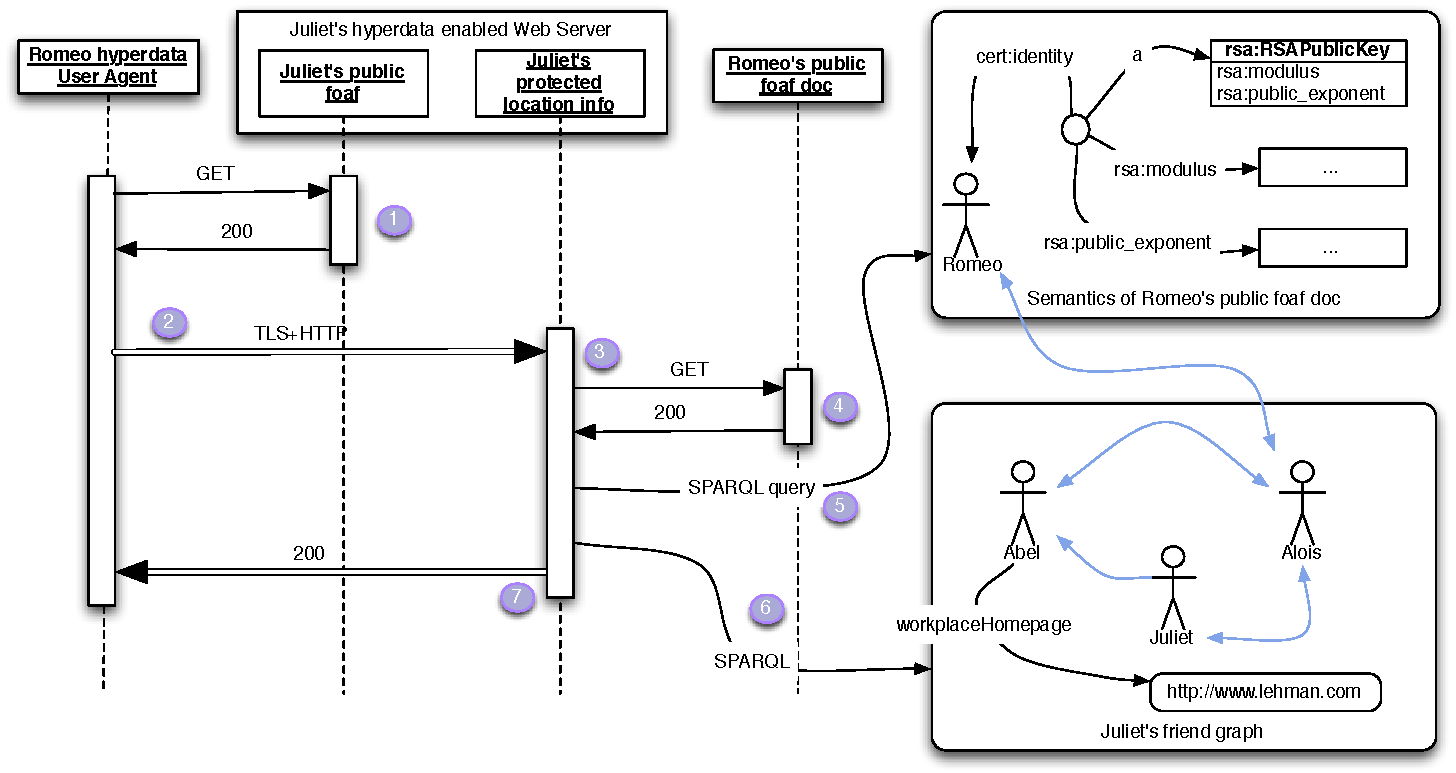
\includegraphics[width=\columnwidth]{figures/foaf_ssl_sequence}
\caption{The FOAF+SSL sequence diagram.}
\label{fig:foafsslseqdiag}
\end{figure}

The FOAF+SSL authentication protocol consists of the following steps,
as illustrated in Figure~\ref{fig:foafsslseqdiag}:

\begin{enumerate}
\item A client fetches a public HTTP resource which points to a
  protected resource for example {\tt <https://juliet.example/location>}.
\item The client {\tt romeo:i} dereferences this URL.
\item During the SSL handshake (when the connection is initiated), the
  server requests a client certificate. Because FOAF+SSL does not rely
  on CAs, it can ask for {\em any} certificate.  The client sends
  Romeo's certificate (which may be self-signed) containing its public
  key (see ``{\tt Subject Public Key Info}'' in
  Listing~\ref{listing:x509cert}) and a {\em Subject Alternative Name}
  URI (see ``{\tt X509v3 extensions}'' in
  Listing~\ref{listing:x509cert}).  Because the SSL handshake has been
  successful, Juliet's server knows that Romeo's client has the
  private key corresponding to the public key of the certificate.
\item Juliet's server dereferences the Subject Alternative Name URI
  found in the certificate and fetches an RDF document.
\item The document's {\em log:semantics} is queried for information
  regarding the public key contained in the X.509 certificate
  mentioned previously.  This can be done in part with a SPARQL query
  as shown in Listing~\ref{listing:sparqlpub}.  If the public key of
  the certificate is found to be identical to the one published in the
  FOAF file, this proves that the client is using the URI correctly.
\item Once this fundamental authentication step is complete, Romeo's
  identity (as represented within the server) may also be augmented
  with information regarding its position in a graph of relations
  (including friendship ones), in order to determine a degree of trust
  according to some criteria. Juliet's server can get this information
  by crawling the web starting from her FOAF file, or by other means.
\item Authentication has been done; authorization can now take place.
\end{enumerate}

\begin{lstlisting}[basicstyle=\rm\scriptsize\ttfamily,label={listing:x509cert},caption={Excerpt of a text representation of a FOAF+SSL certificate.}]
     Subject Public Key Info:
            Public Key Algorithm: rsaEncryption
            RSA Public Key: (1024 bit)
                Modulus (1024 bit):
                    00:b6:bd:6c:e1:a5:ef:51:aa:a6:97:52:c6:af:2e:
                    71:94:8a:b6:da:9e:5a:5f:08:6d:ba:75:48:d8:b8:
                    [...]     
                Exponent: 65537 (0x10001)
     X509v3 extensions:
           X509v3 Subject Alternative Name: 
                           URI:https://romeo.example/#i
\end{lstlisting}

\begin{lstlisting}[basicstyle=\rm\scriptsize\ttfamily,label={listing:sparqlpub},caption={SPARQL query to obtain the public key information.}]
SELECT ?modulus ?exp WHERE { 
   \?key cert:identity <https://romeo.example/#i>;
        a rsa:RSAPublicKey;
        rsa:modulus [ cert:hex ?modulus; ];
        rsa:public_exponent [ cert:decimal \?exp ] .   }            
\end{lstlisting}

\subsection{Authentication Logic}
\label{sec:authlogic}

This section draws a parallel with Section~\ref{sec:tlsauth}, again,
following the reasoning of the web server {\tt S} in giving {\tt
  \_:client} access to some resource {\tt R}.

At the end of stage 3 in the FOAF+SSL sequence diagram, the server
{\tt S}, has received the client certificate securely. Being
self-signed (or signed by an unknown party), its semantics are
somewhat different. Furthermore, what interests {\tt S} in this
FOAF+SSL certificate are only the URI identifiers to refer to the
subject, abandoning thus the limitations of DNs. In addition, since it
is asserted by the client, {\tt S} knows that:\footnote{The signer
  being the author, following the reasoning from
  P\ref{prop:foafCertClientClaim}, P\ref{prop:sigverif},
  D\ref{def:signedCertClaim} would also end up with this result ---
  for self signed certificates only.}

\begin{customprop}{prop:foafCertClientClaim}
\begin{verbatim}
 _:client :claims _:clientGrph .
 _:clientGrph =  { <> dc:created romeo:i; foaf:primaryTopic romeo:i.
                   romeo:i hasPrivateKeyFor pubKey .  } 
\end{verbatim}
\end{customprop}


{\tt S} may know nothing of {\tt romeo:i}. However, it knows from the
TLS session that:

\begin{customprop}{prop:foafPubKey}
\begin{verbatim}
 _:client :hasPrivateKeyFor pubKey . 
\end{verbatim}
\end{customprop}

Now when someone makes a claim, it is understood that they have to abide by
the consequences of their claim. But also that they have to agree to the consequences
of their claims with new facts put to them.  So someone who makes a claim {\tt :mustAgree} 
with anything we know securely, and the consequences of what they believe and what
we know. We can write this out as the following rule:

\begin{customprop}{prop:mustAgree}
\begin{verbatim}
 {  ?client :claims ?clientGraph . 
  ( ?clientGrph   secureFactGraph   owlReasoningRules ) 
     log:conjunction [ log:conclusion ?C ] }
              => { ?client :mustAgree ?C  } 
\end{verbatim}
\end{customprop}

Hence, it from P\ref{prop:foafCertClientClaim},
P\ref{prop:foafPubKey}, and D\ref{def:hasPrivateKeyFor} that {\tt
  \_:client} would have to agree with it that it is {\tt
  romeo:i}. This should not be a surprise, as that is indeed what
one assumes someone who sends such a certificate intends.

\begin{customprop}{prop:client_IamClient}
\begin{verbatim}
 _:client :mustAgree [ log:includes { romeo:i = _:client  }  ] .
\end{verbatim}
\end{customprop}

Thus, since {\tt \_:client} asserts it is {\tt romeo:i}, it can find
no harm in {\tt S} finding more information about itself by looking at
{\tt romeo:i}. {\tt S} can do that, as {\tt romeo:i} is a
dereferenceable URI, whereas {\tt \_:client} and {\tt pubKey} are not. So by dereferencing
{\tt romeo:i}, {\tt S} knows that:

\begin{customprop}{prop:foafRomeoSt}
\begin{verbatim}
 romeo:i :semantics _:romeoGrph . 
 _:romeoGrph => { romeo:i hasPrivateKeyFor pubKey } .
\end{verbatim}
\end{customprop}

Again, by P\ref{prop:foafRomeoSt}, P\ref{prop:foafPubKey},
D\ref{def:hasPrivateKeyFor}, and P\ref{prop:mustAgree}:

\begin{customprop}{prop:romeo_IamClient}
\begin{verbatim}
 :romeo:i :mustAgree [ log:includes { romeo:i = _:client  }  ] .
\end{verbatim}
\end{customprop}

In other words, both {\tt romeo:i} and {\tt \_:client} must agree,
given what {\tt S} knows, that {\tt S} can consider {\tt romeo:i
  owl:sameAs \_:client}.  In particular {\tt romeo:i} cannot repudiate
this assertion since {\tt romeo:i} itself provided
P\ref{prop:foafRomeoSt} authoritatively. It follows that if {\tt S} is
authorized to serve {\tt R} to {\tt romeo:i}, {\tt S} can serve {\tt
  R} to {\tt \_:client}.

%In other words, both {\tt romeo:i} and {\tt \_:client} would agree,
%given what {\tt S} knows, that they are the same. The advantage of
%this reasoning via an indirection of what others would have to agree
%to given what S knows, is that it allows {\tt S} to assert the
%minimum it needs to, and so be minimally liable.

%It follows then that if {\tt S} has to serve R to {\tt romeo:i} then
%{\tt romeo:i} cannot disagree if {\tt S} serves {\tt R} to {\tt
%\_:client}; this is all {\tt S} needs to know to accomplish its task.

%It is an interesting further question to find out if S also knows
%that {\tt romeo:i = \_:client}, but we have not at present had enough
%time to look into this.
\subsection{Following links}
\label{sec:LinkCrawling}

In the previous section we showed how a server can grant
access to a resource to a client who claims a WebId.  How to decide
which group of Agents has access to the resource will be for each
application to decide. It could be done just by listing resources --
as one could do if one knew the WebIds of all one's friends.  It could
be done by trusting statements returned by a selected group of WebIds,
such as when allowing all friends of one's friends access to a
resource, as specified by the representation returned by their
WebId. This would make the initial list of WebIds similar to the PKI  trust anchors.
 The decision of what rule to follow to serve up a resource is very much 
 up to its owner, and is a field where a lot still remains to be tried out.

A topic for further research is to define the various ways in which
trust can be transmitted. Let us look at one simple example
here. Imagine a user connects to a service and is authenticated as
{\tt joe:i}, using the FOAF+SSL method described above. Imagine {\tt
  joe:i} returns a representation claiming {\tt joe:i owl:sameAs
  romeo:i}. Since anyone could make that statement that in itself
should not be the basis for belief for services that care about
security. If, on the other hand, {\tt romeo:i :semantics [
    log:includes \{ romeo:i owl:sameAs joe:i . \} ]}, then this could be
used as confirmation of the claim, and from there on both Ids could be used 
interchangeably by {\tt S}.

\section{Related work}
\label{sec:other}

%FOAF+TLS builds on
%a number of existing proposals and implementations of various authentication
%systems. More specifically, FOAF+TLS relies on the TLS layer to authenticate the client (that is, to verify that 
%the remote client is indeed in possession of the private key corresponding to this certificate)
%and on the Web to authenticate the identity claim made by the client in its certificate.

Unlike the OpenPGP extension to TLS~\cite{rfc5081}, which also aims to
rely on a web-of-trust by using PGP certificates instead of the usual
X.509 certificates, FOAF+SSL makes only slight changes in the way
X.509 certificates are used; it does not require changes in the actual
SSL stack. With the OpenPGP TLS extension, the problem of key
distribution still remains, whereas FOAF offers more flexibility in
that respect.

OpenID also shares considerable similarities with FOAF+SSL, due in
part to OpenID's reliance on URLs as identifiers, just as FOAF+SSL
relies on dereferenceable URIs bearing FOAF data. However, it fails to
make much use of the information at the OpenId resource, using it only
to find the authorization service. As a result, OpenID requires a much
higher number of connections to establish identity --- 6 as opposed to
2 --- and parts ways with RESTful design in the attribute exchange
spec, loosing thereby the advantages of a networked architecture.

\section{Conclusions}

FOAF+SSL provides a secure and flexible way to have a global
authentication system.  Through the use of public key cryptography, it
increases security compared with other approaches such as OpenID.  In
addition, the use of public key certificates may help verify more
properties in the FOAF-based web-of-trust.  FOAF+SSL is also RESTful
and integrates well with the Semantic Web.  Compared with PKI,
FOAF+SSL removes the need for hierarchical authorities for asserting
identity making it more flexible and less bureaucratic.  Thus, this
mechanism adapts itself well to the formation and expansion of virtual
organisations and distributed social networks.

\bibliographystyle{splncs}
\bibliography{spot2009,rfc}


\end{document} 
